\section{Filtro AR}

\subsection{Función \textit{positiveSpectrum}}

Se implementa la función \textit{positiveSpectrum(x)} que recibe como entrada una señal digital \textit{x}, de largo $N$, la cual haciendo uso de la función \textit{fft()}  de Matlab pueda entregar el vector \textit{amp} que corresponde  de amplitudes de la DFT  para el rango de frecuencias positivas y un vector \textit{w} correspondiente a las frecuencias normalizadas en \textit{rad/muestra}. El código de la función descrita se presenta a continuación


\begin{lstlisting}[language = octave]
function [amp,w] = positiveSpectrum(x)
    X = fft(x);
    amp = X(1:floor(length(X)/2))
    w = linspace(0,pi,length(amp))
end

\end{lstlisting}

Para poner a prueba la función implementada se grafica usando el comando  \texttt{plot()} el espectro en frecuencia positivo de la vocal \textit{A} contenida en la señal \textit{vowel\_a}, obteniendo la gráfica presente en la figura \ref{frec_A_positive}

\begin{figure}[H]
    \centering
    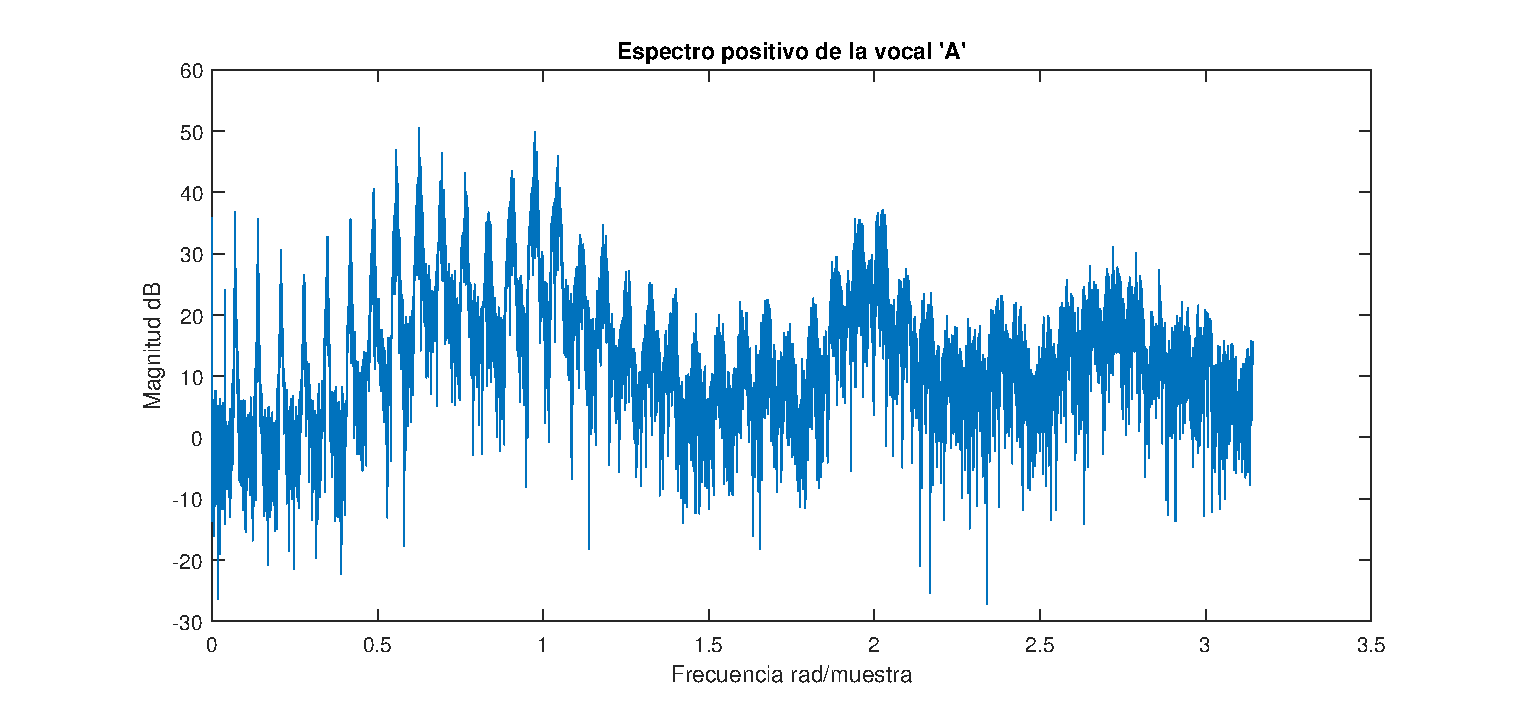
\includegraphics[scale = 0.5]{figures/4_1_espectroA.eps}
    \caption{Espectro de la señal \textit{vowel\_a}}
    \label{frec_A_positive}
\end{figure}

En el espectro obtenido se pueden diferenciar 4 formantes ubicadas aproximadamente en $0.6$, $1.2$, $2$ y $2.7 ~rad/muestra$ 
\subsection{Experimentación con Órdenes del filtro AR en LPC}

Para está parte se utiliza el código \texttt{p4\_2.m}, el cual se adjunta a la entrega.

Inicialmente se gráfica de la respuesta en frecuencia del filtro AR de orden 15 y 2, junto al espectro de $vowel\_a$. Los gráficos se muestran en la figura \ref{fig:p4_21}. Se aprecia que con 2 polos se tiende a formar una resonancia al medio de los 2 formantes de la vocal. 

\begin{figure}[H]
    \centering
    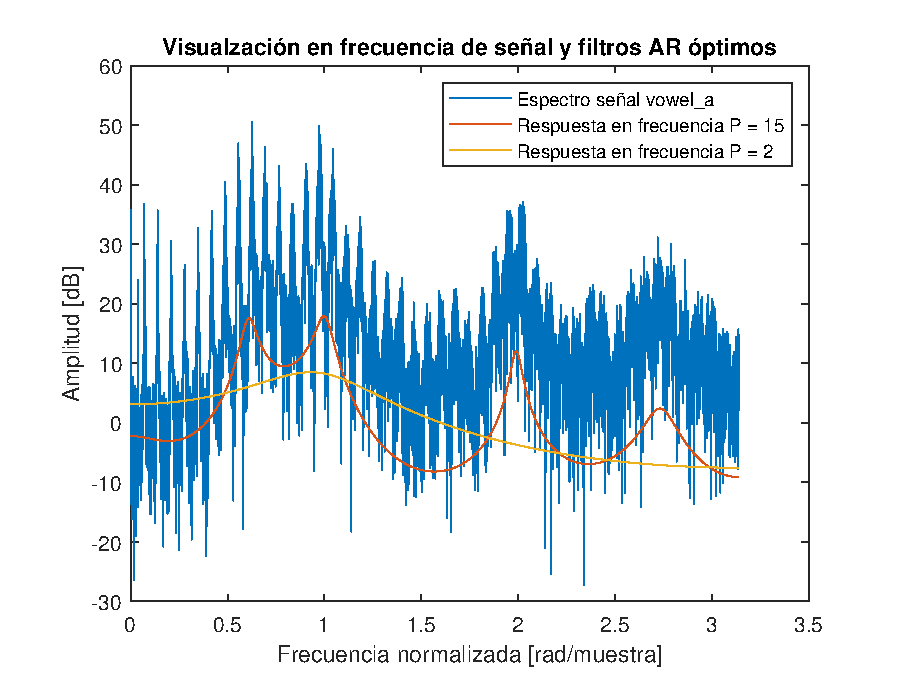
\includegraphics[width = .8\linewidth]{figures/p4_2arbajo.eps}
    \caption{Espectro de $vowel\_a$ y respuesta en frecuencia del filtro AR de orden 15 y 2 obtenidos por LPC.}
    \label{fig:p4_21}
\end{figure}

Por otro lado se obtiene el diagrama de polos y ceros de los filtros diseñados para la vocal a. Dichos diagramas se muestran en la figura \ref{fig:p4_22}

\begin{figure}[H]
    \centering
    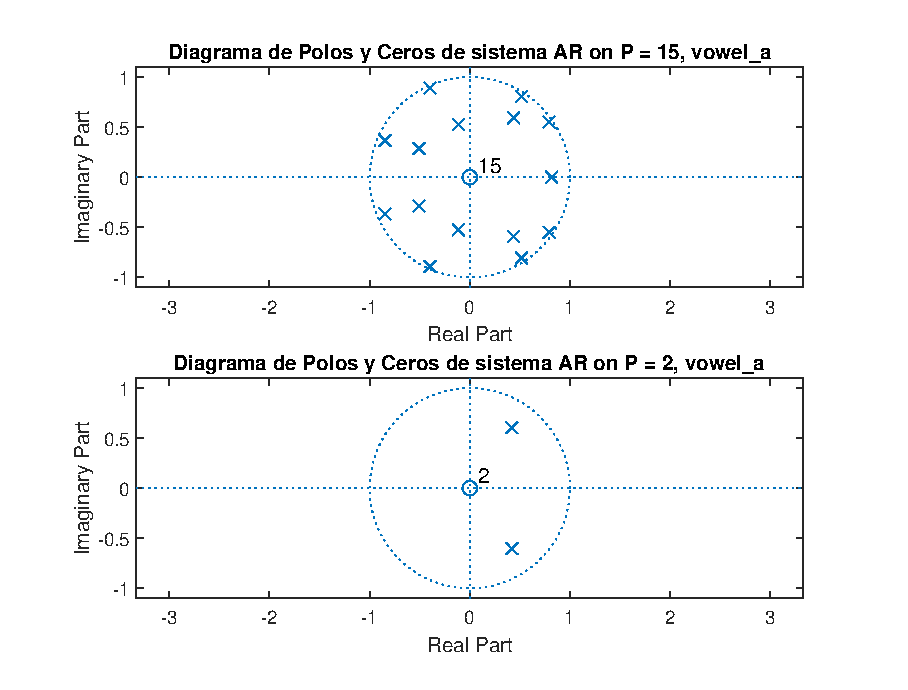
\includegraphics[width = .8\linewidth]{figures/p4_22.eps}
    \caption{Diagrama de polos y ceros para filtros de orden 15 y 2 diseñados por LPC para la señal $vowel\_a$.}
    \label{fig:p4_22}
\end{figure}

Posteriormente se grafica de la respuesta en frecuencia del filtro AR de orden 15 y 2, junto al espectro de $vowel\_u$, los cuales se muestran en la figura \ref{fig:p4_23}. Se aprecia que con 2 polos se tiende a formar una resonancia en la frecuencia 0. Lo anterior también se aprecia en la figura \ref{fig:p4_24}, donde se presenta el diagrama de polos y ceros para los filtros diseñados para la vocal u.

\begin{figure}[H]
    \centering
    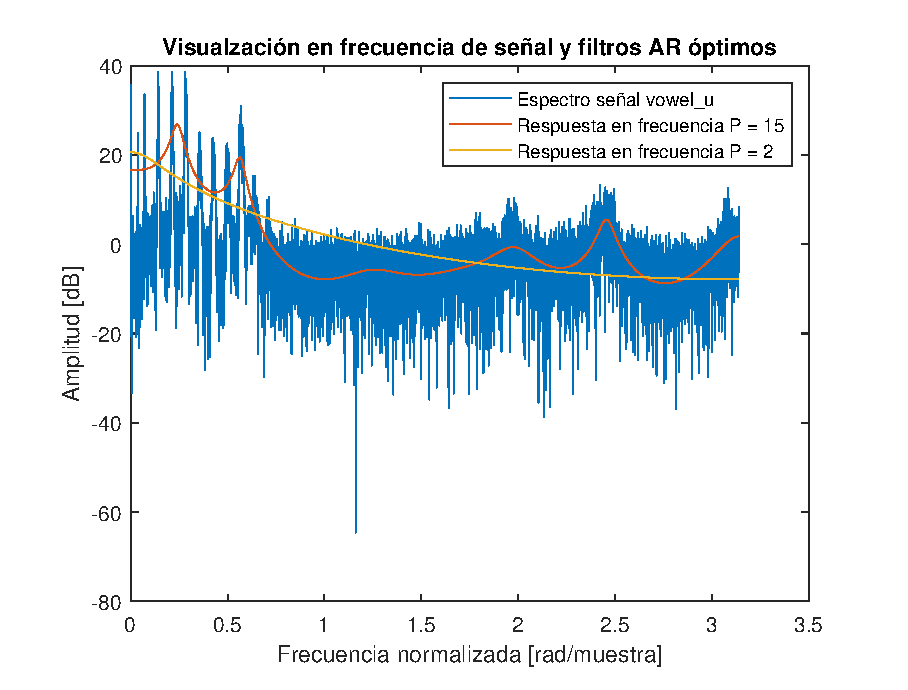
\includegraphics[width = .8\linewidth]{figures/p4_23.eps}
    \caption{Espectro de $vowel\_u$ y respuesta en frecuencia del filtro AR de orden 15 y 2 obtenidos por LPC.}
    \label{fig:p4_23}
\end{figure}

\begin{figure}[H]
    \centering
    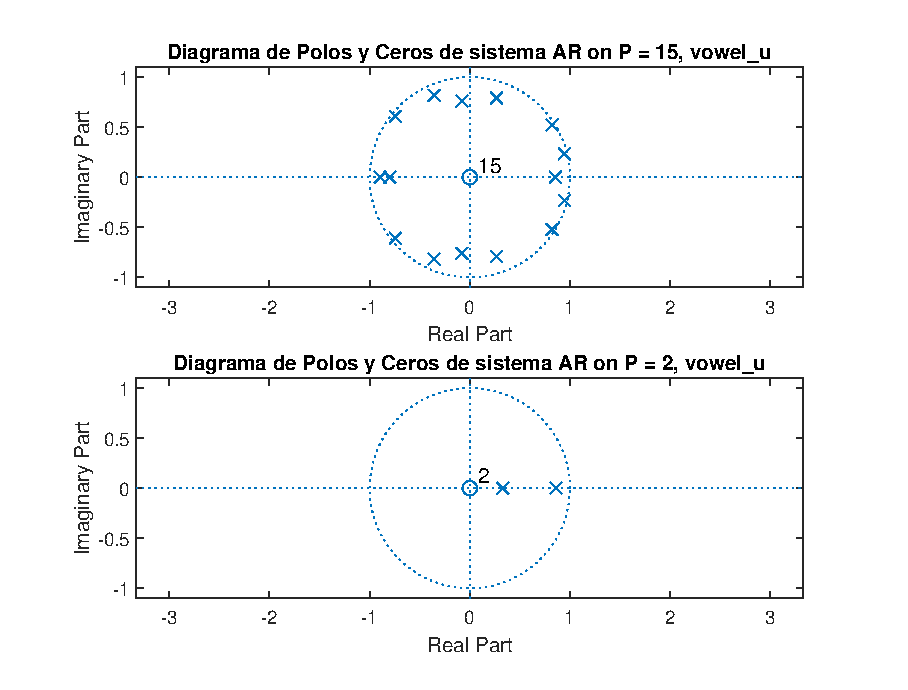
\includegraphics[width = .8\linewidth]{figures/p4_24.eps}
    \caption{Diagrama de polos y ceros para filtros de orden 15 y 2 diseñados por LPC para la señal $vowel\_u$.}
    \label{fig:p4_24}
\end{figure}



%%%%%%%%%%%%%%%%%%%%%%%%%%%%%%%%%%%%%%%%%%%%%%%%%%%%%%%%%%%%
\subsection{Comparación de filtrado AR de distinto orden}

Para estudiar las diferencias de resultados al filtrar una señal con filtros AR de distinto orden, primero se escoge una señal de vocal arbitraria para que sea filtrada, en este caso se escogió la señal \textit{vowel\_a} correspondiente a la vocal \textit{A}.

Lo siguiente es definir los ordenes de los filtros que se usarán, se escoge como referencia un orden relativamente alto 15 y uno menos de 9. Se crea un tren de impulsos de $100~Hz$ de frecuencia  con $0.5~s$ de duración. Se obtienen los coeficientes $a_k$ de cada filtro y se procede con el filtrado de la señal.

Los resultados obtenidos se muestran en las gráficas de la figura \ref{AR-15-9}, se incluyen además los diagramas de polos y ceros en la figura \ref{zplane1}, donde la gráfica superior corresponde al diagrama asociado al filtro de orden 15 y la inferior al filtro de orden 9.


\begin{figure}[H]
    \centering
    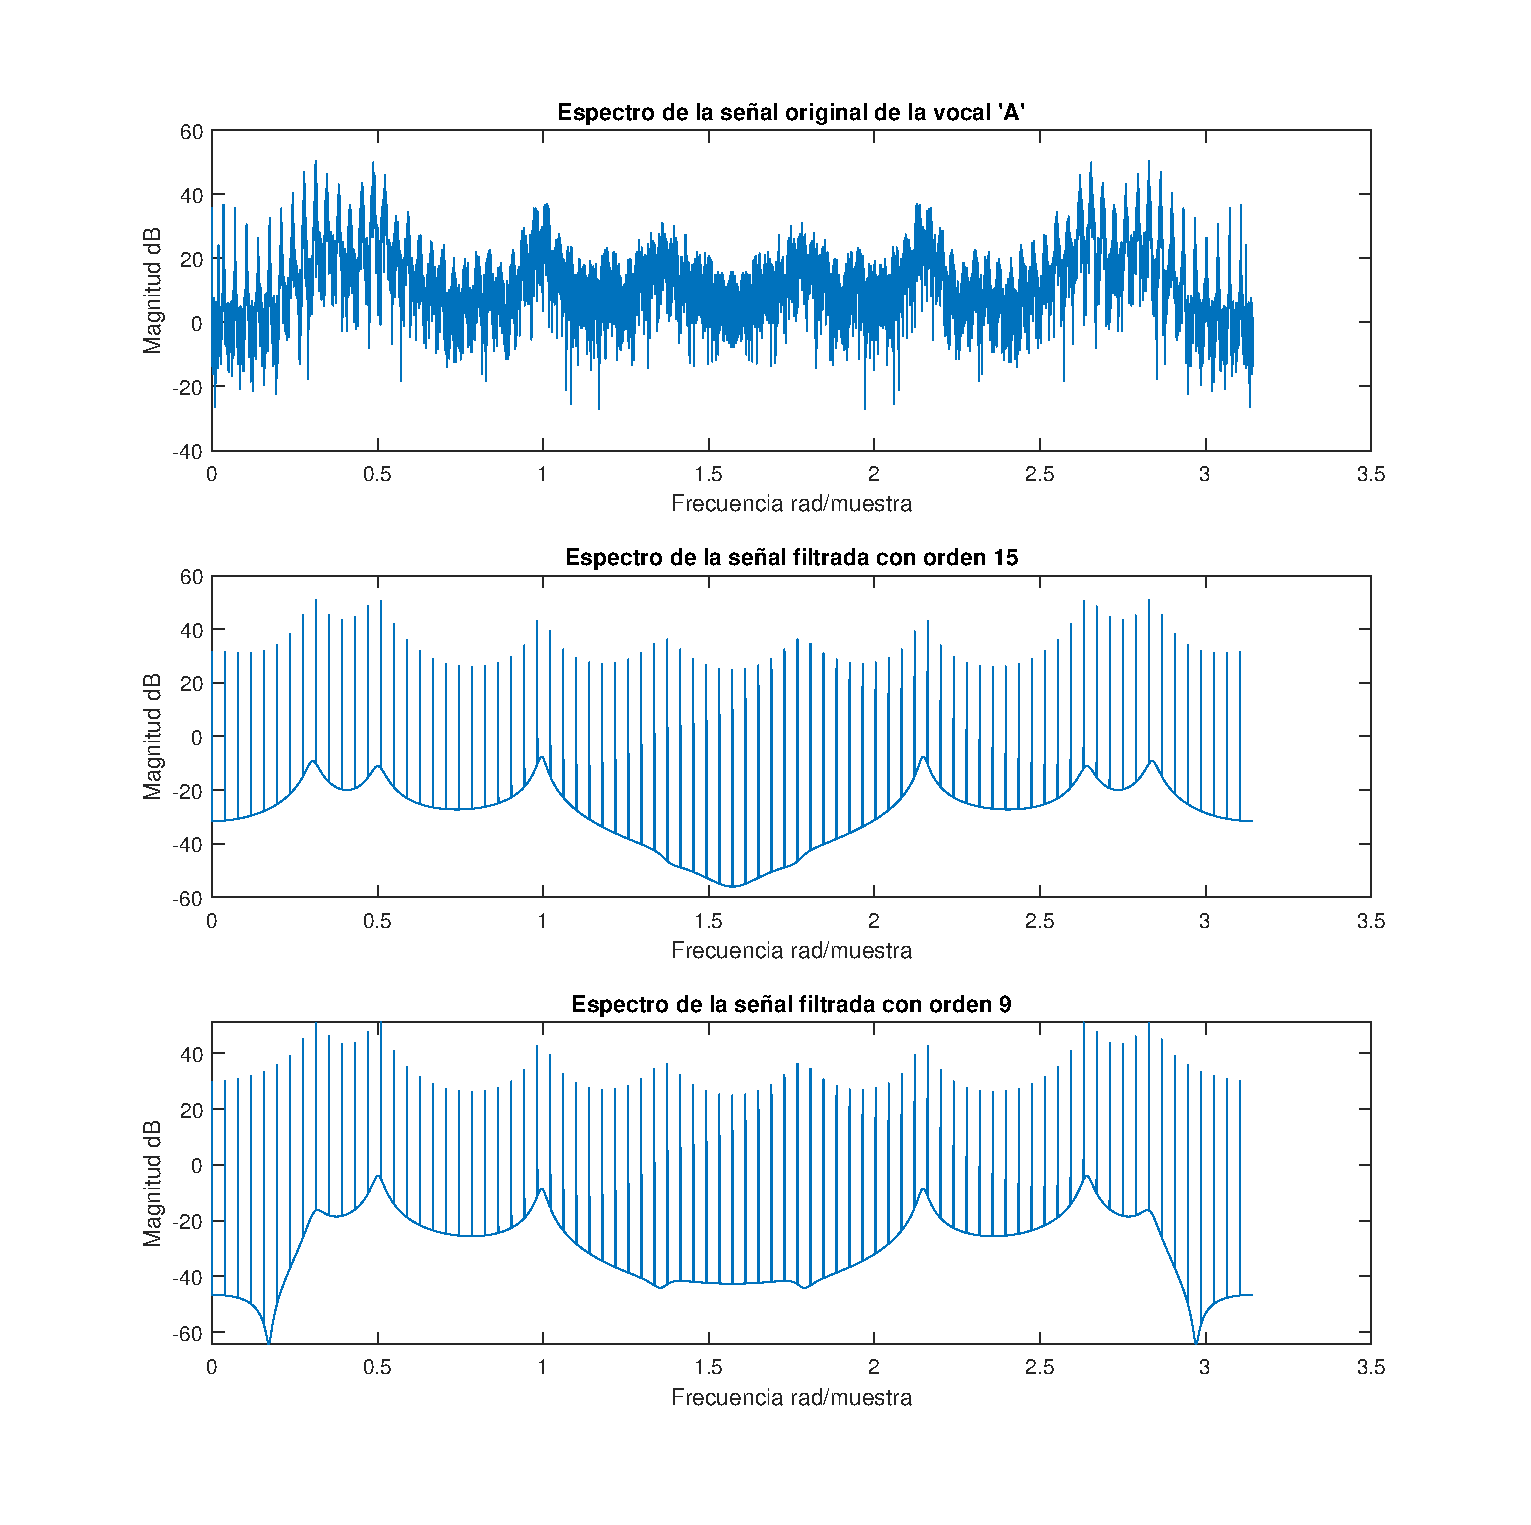
\includegraphics[scale = 0.6]{figures/4_3_filtradoAR.eps}
    \caption{Espectro en frecuencia de la señal \textit{vowels\_a} y el resultado de filtrado de orden 15 y 9 }
    \label{AR-15-9}
\end{figure}

\begin{figure}[H]
    \centering
    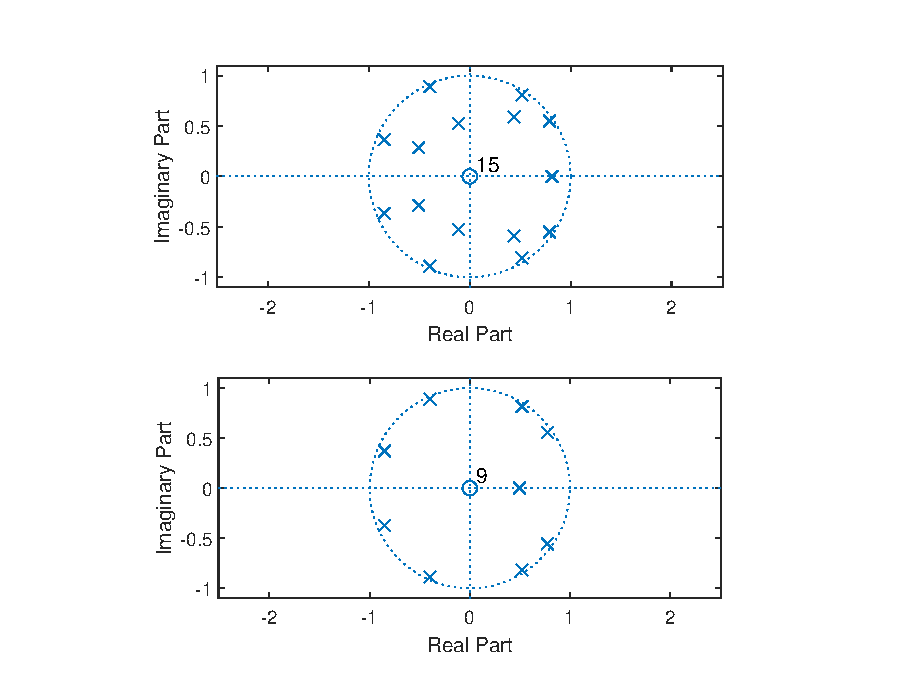
\includegraphics[scale = 0.9]{figures/4_3_zplane1.eps}
    \caption{Diagramas de polos y ceros para los filtros AR de orden 15 y 9}
    \label{zplane1}
\end{figure}


Se pide además realizar el mismo ejercicio anterior comparando el filtrado de la señal \textit{vowel\_u} correspondiente a la vocal \textit{U}, probando distintos ordenes de filtrado hasta encontrar el mínimo orden que no presente diferencias significativas en cuando a la percepción auditiva  respecto al resultado obtenido con el filtrado de orden 15. 

Se notó que haciendo uso de un filtro de orden 10 la señal ya se distorsiona lo suficiente para tener la impresión de que la vocal está siendo emitida por una persona distinta, por lo que se concluye que el orden mínimo para no tener diferencias significativas un filtro de orden 11. Los espectros en frecuencia obtenidos para filtros de orden 15 y 10 se presentan en la figura \ref{AR-15-10},  se incluyen además los diagramas de polos y ceros en la figura \ref{zplane2}, donde la gráfica superior corresponde al diagrama asociado al filtro de orden 15 y la inferior al filtro de orden 10.

\begin{figure}[H]
    \centering
    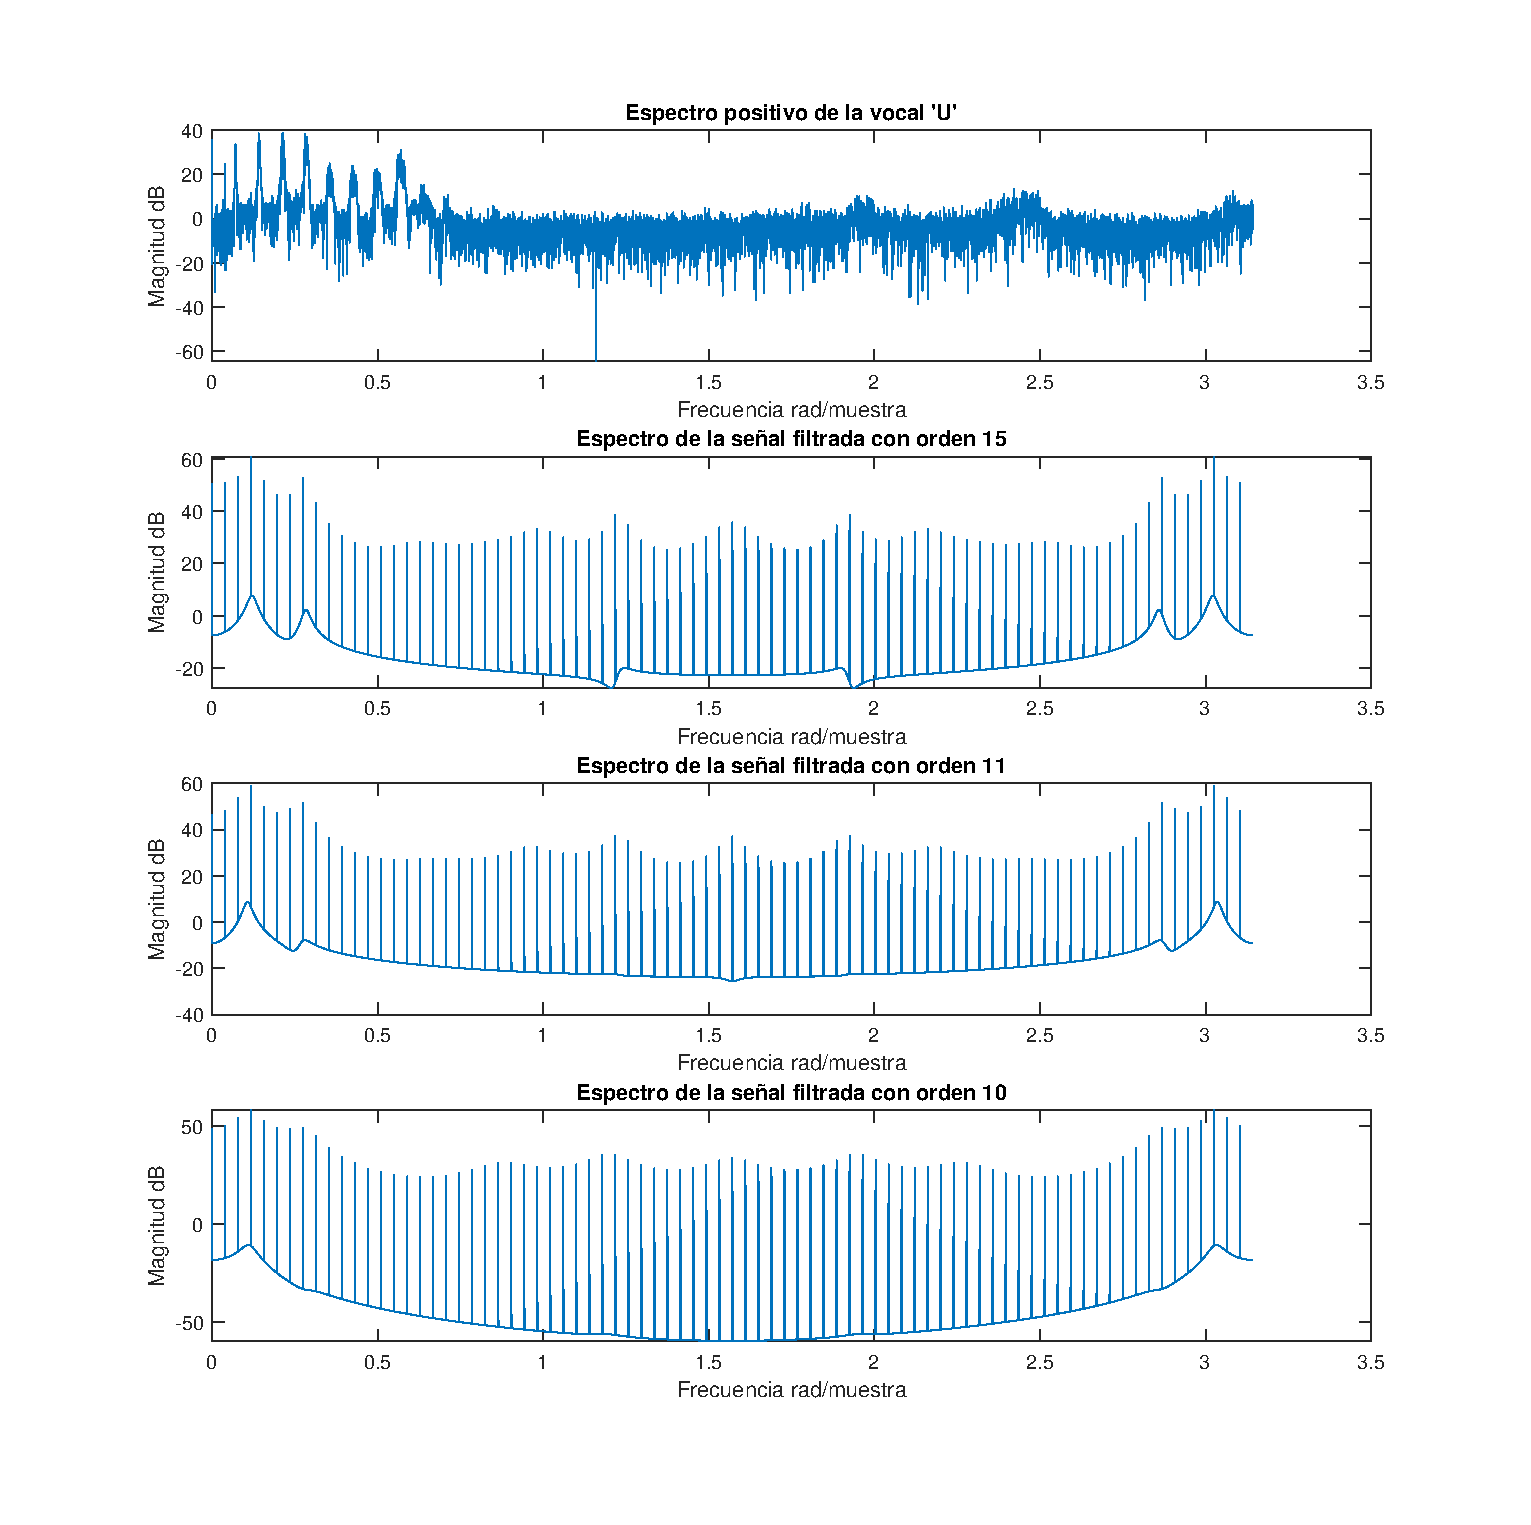
\includegraphics[scale = 0.5]{figures/4_3_filtradoU.eps}
    \caption{Espectro en frecuencia de la señal \textit{vowels\_u} y el resultado de filtrado de orden 15 y 10 }
    \label{AR-15-10}
\end{figure}

\begin{figure}[H]
    \centering
    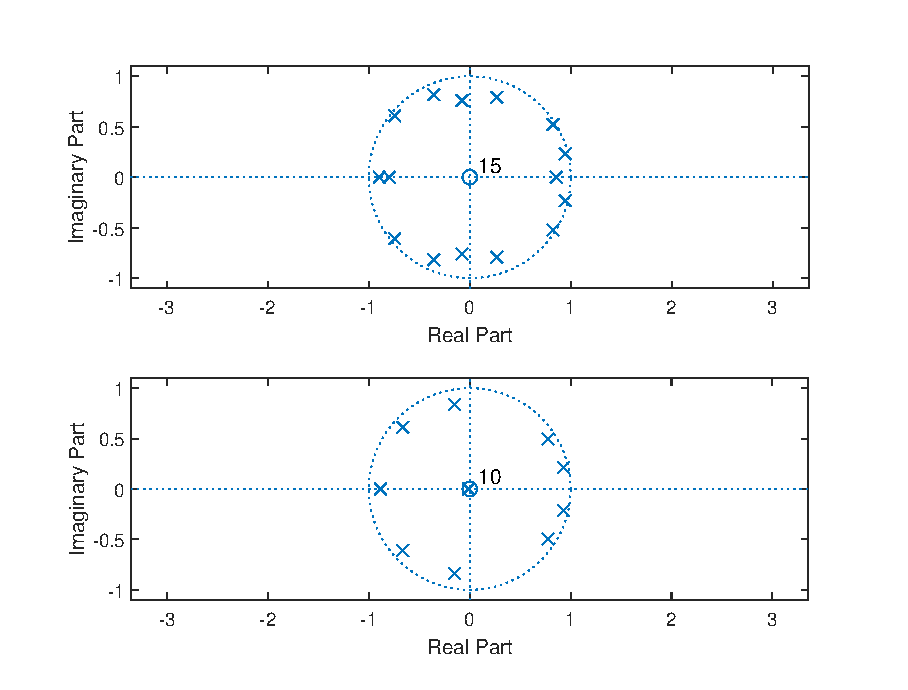
\includegraphics[scale = 0.8]{figures/4_3_zplaneu.eps}
    \caption{Diagramas de polos y ceros para los filtros AR de orden 15 y 10}
    \label{zplane1}
\end{figure}


De la figura \ref{AR-15-10} se puede ver que en el espectro de la vocal \textit{U} se ven 5 formantes, y el orden mínimo que permitía una síntesis de la señal sin diferencias significativas fue 11. Por otro lado en en la figura \ref{frec_A_positive} de la sección 4.1 se encontraron 4 formantes y cuando se sintetizó la señal con un filtro de orden 9 no se notaron diferencias significativas respecto al filtrado de orden 15, con esto se puede concluir que un buen criterio para lograr una buena síntesis de este tipo de señales es encontrando el orden según $2n + 1$, siendo $n$ el número de formantes de la señal a sintetizar.
%%%%%%%%%%%%%%%%%%%%%%%%%%%%%%%%%%%%%%%%%%%%%%%%%%%%%%%%%%%%
\subsection{Filtro AR con filtros \textit{ \textit{Biquad}}}

El procedimiento que hasta ahora se ha  llevado a cabo haciendo uso de filtros AR de distintos ordenes se puede homologar mediante el procesamiento en cascada de la señal con múltiples filtros \textit{ \textit{Biquad}} como los estudiados en experiencias anteriores. Matlab provee de la función  \texttt{tf2sos(b,a)} que recibe como parámetros los coeficientes $a_k$ y $b_k$ de un filtro y entrega la matriz sos, que contiene en sus $n/2$ filas en caso de que n sea par y $n/2 + 1$, donde n corresponde al orden del filtro original. Cada fila contiene los coeficientes del numerador y denominador $A_k$ Y $B_k$ de los filtros \textit{\textit{ \textit{Biquad}}} necesarios para que, de en forma de cascada filtren una señal y obtengan el resultado del filtro original. El comando además entrega el  parámetro \textit{g} correspondiente a la ganancia que poseen los filtros \textit{\textit{ \textit{Biquad}}}  entregados en la matriz.


Se experimenta el uso de la función  antes descrita para un filtro AR de orden 15 obtenido al usar el comando \texttt{lpc} para la señal \textit{vowel\_a}, se obtiene la respuesta en frecuencia de cada filtro  \textit{Biquad} entregado en la matriz permitiendo analizar el aporte individual de cada una de ellas en la respuesta en frecuencia total. Se grafican dichas respuestas en frecuencia  forma superpuesta como se puede ver en la figura \ref{Biquads}.


\begin{figure}[H]
    \centering
    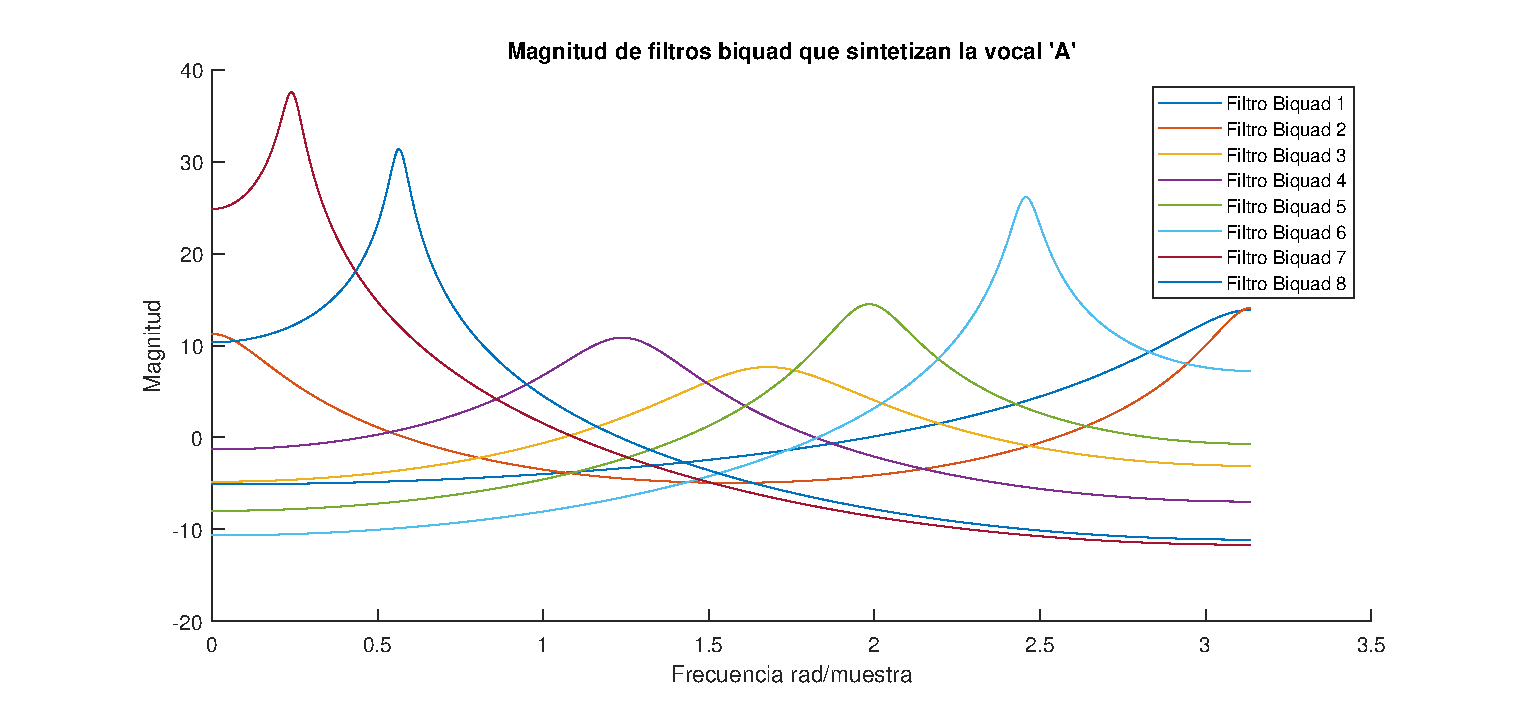
\includegraphics[scale = 0.6]{figures/4_4.eps}
    \caption{Magnitud en $dB$ de la respuesta en frecuencia de los filtros \textit{ \textit{Biquad}} entregados por la función \texttt{tf2sos(b,a)}}
    \label{Biquads}
\end{figure}


Se grafican además de forma superpuesta las magnitudes de las respuestas en frecuencia de los filtros junto al espectro de la señal \textit{vowel\_a} como se muestra en la figura \ref{Biquadss_vocal}

\begin{figure}[H]
    \centering
    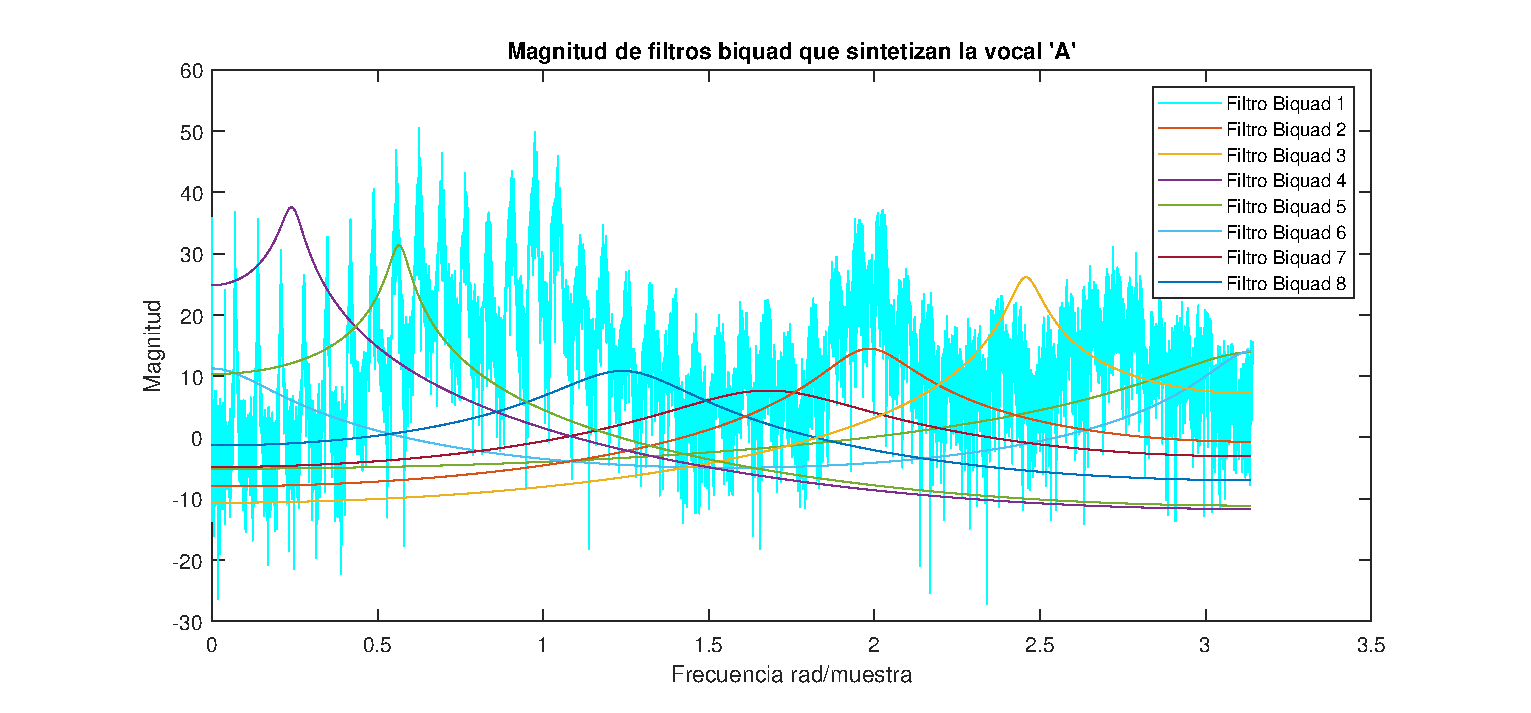
\includegraphics[scale = 0.6]{figures/4_4_vocal.eps}
    \caption{Magnitud en $dB$ de la respuesta en frecuencia de los filtros \textit{ \textit{Biquad}} entregados por la función tf2sos(b,a) junto al espectro de la vocal \textit{A}}
    \label{Biquadss_vocal}
\end{figure}





